\section*{}

% \begin{auxmulticols}{1}
%     \lipsum[1-2]
% \end{auxmulticols}

\begin{center}
    \textit{This work is dedicated to my mentor and my friend Noel White, (1951-2021).}
\end{center}

\section{Introduction} \label{sec:intro}

Open clusters have been shown to be an integral part of the astronomer's toolbox, readily lending themselves as stellar laboratories. Open clusters are classified as a group of stars around the same age and loosely bound through mutual gravitation. \\
Their similar age allows for in-depth observation of the stellar evolution. Through this, many attributes of the stellar population can be inferred. As clusters span age ranges from a couple of Myr to Gyrs, many have been present since the formation of the disk itself. Through this, if clusters of varying ages are examined, it is possible to trace the evolution of the milky way.  \\

Mapping the milky way has always been difficult, given the vantage point it can be observed from. This makes it quite challenging to appreciate the shape and dimensions of the milky way. Some of the pioneering studies, such as \cite{1785RSPT...75..213H,1918ApJ....48..154S} and \cite{1930LicOB..14..154T} first outline the use of open clusters to map the galaxy. Following with studies like \cite{1970IAUS...38..205B} which pathed the spiral arms of the milky way using open clusters and numerous studies by \cite{1958ZA.....46..176V} which explore the evolution of the galaxies scale height. \\

To more recent studies such as \cite{2006Bon}. Which use young open clusters to predict shape evolution of the galaxy, by analysing to longitudal distribution of young clusters to predict reflect on areas of star formation and presence of spiral arms. 

While the precision and accuracy of cluster age estimates are tied to the quality of the observational data and theoretical models, the process of estimating cluster age through the use of colour-magnitude diagrams is relativity straightforward and has been shown to be tried and true. Even early open cluster catalogues like \cite{1988ESOC...28..379L} included distance estimates, while more recent catalogues like \cite{2008A&A...486..771K} have provided other parameters such as age, metallicity and excess colour. Furthermore, with the second data release from Gaia \citep[GDR2;][]{2018A&A...616A...1G}. 
presents the most in-depth all-sky astrometric and photometric study to date. \\

This increase in available data has allowed for the characterisation of open clusters on mass adding to catalogues such as WEBDA. Determination of all open clusters identified by Gaia is an ongoing task and is being automated using modern techniques and machine learning as shown in studies by \cite{2019A&A...623A.108B} and \cite{2020A&A...640A...1C}. \\

\\ 

This study used the 1.25 m optical telescope at the Calar Alto Observatory (CAHA) to observe four open clusters from the WEBDA catalogue. The aim of this work was to classify the four observed clusters and infer details of each cluster. Then use this observational cluster classification in tandem with other open clusters from the WEBDA catalogue to trace the paths of clusters in the galactic disk, studying both its structure and evolution.


% \section{Targets}



\section{Observations} 

This study observed 4 open-clusters from the WEBDA database on the night of March 10th 2022. Each cluster was observed using B and V filters in the Johnson Cousins' UBVI system. The average observation time for each cluster was X with image calibration and reduction carried out. 

\subsection{Target Selection Strategy}

For this work it was important for the sample to observe clusters grouped at a similar area of the galactic disk (see. \cref{fig:TargetSelection}) at varying estimated cluster ages, with each group containg an old ($>1000$ Myr), young ($<100$ Myr) and one intermediate cluster. In grouping the targets like this it would allow for comparison between galactic position of and varied age, giving the most to the small quanitiy of clusters analysed. \\ The observed targets are listed in \cref{tab:target_list}. A further six open clusters from the WEBDA catalog are also analysed to add to the sample size of clusters analysed and classified by the methods of this work. The six cluster were intailly propsed for observation but not-observed due to poor conditions during the observation period. 


\begin{deluxetable*}{lccr}[ht]
  \tablecaption{List of analysed targets. \label{tab:target_list}}
  \tablehead{
  \colhead{Target Cluster} & \colhead{RA (J2000)} & \colhead{DEC (J2000)} & \colhead{WEBDA Study} \\ 
\colhead{} & \colhead{hh:mm:ss} & \colhead{deg:mm:ss}  &   
  }
  % \decimalcolnumbers
  % \tablewidth{}
  \startdata
  Berkeley 28  & 06:52:12  & 02:56:00   & \cite{1988Mohan}  \\ 
  Bochum 2 & 06:48:54 &  00:23:00  & \cite{1993Turbide} \\ 
  NGC2324 & 07:04:07  & 01:02:42   & \cite{1998Frandsen} \\
  NGC2355 & 07:16:59  &  13:45:00  & \cite{1991Kalunzy} \\ \hline 
  \multicolumn{4}{c}{\textit{Proposed Open Clusters}} \\ \hline
  Berkeley 20 & 05:33:00 & 00:13:00 & \cite{2001Durgapal} \\ 
  Berkeley 34 & 07:00:24 & -00:15:00 & \cite{2005Ortolani} \\ 
  King 1 & 00:22:04 & 64:22:50 & \cite{2004Lata} \\ 
  King 15 & 00:32:54 & 61:52:00 & \cite{1994Phelps} \\ 
  NGC 2129 & 06:00:41 & 23:19:06 & \cite{2006Carraro} \\ 
  Stock 18 & 00:01:37 & 64:37:30 & \cite{2012Bhatt} \\ 
  \enddata
  \tablecomments{Above details the targets analysed throughout this work. The first four targets were obsereved at CAHA. With the following six grouped as the proposed clusters. The associated WEBDA study used for supplementation is also listed.}
\end{deluxetable*}




\subsection{Photometry}
Photometric analysis was carried out by first using \verb|DAOStarFinder| with a FWHM chosen taken as the average of moderate sources to favour an array of sources. Aperture photmetry performed as standard. To try make the most of the detected sources an trial apertures were taken on each source locating the aperture that corresponded to the highest SNR value. The aperture for each max SNR value was noted, with the final used aperture value used was taken to be the mean value of all sources apertures that did not exceed a SNR value of 50 or greater. Much like the choice around the FWHM value this choice was used to optimise the magnitudes attained for all detected sources. 

\subsubsection{Magnitude Calibration}

The instrumental magnitude was calibrated to the real magnitude using 9th data release of the AAVSO Photometric All Sky Survey (APASS9). Each source was queried to the APASS9 catalog if a source in the catalog was witin 3 pixels (1.806 arsecs) of source centroid position the query was considered a match and respective real $(\mreal)$ and instrumental magnitudes $(\minst)$ saved. \\ A linear relationship was formed between $\mreal$ and $\minst$ and used for instruemntal conversion.

\subsubsection{Error on Magnitude}

As this study also catalogs 4 clusters it was important to quanitfy error on each of collected magnitude. For this §6 of \cite{bevington_d} was followed closely. This allowed for errors on $\minst$ to be ascribed to $\mreal$ using the deractive and added to quadrature in $\minst$. Then using the full covaraince matrix for propagation through a fitted function gave an error for coverted magnitudes, taking both the APASS error and the error given by SNR $(\Delta M \sim 1/\text{SNR})$

\begin{equation}
  \sigma_{M_{conv.}} = \sqrt{M_{\text{inst.}}^2 \sigma^2_m + \sigma^2_c + 2 M_{\text{inst.}} \sigma^2_{mc}} 
\end{equation}

Where $M_{conv.}$ is the converted magnitude and $m$ and $c$ are the slope and constant the linear fit. The covaraince cross-term $\sigma_{mc}$ was considered negligble due to the internal precision of \verb|numpy.float|.

\section{Population Determination}

The main obstacle in studying open clusters is determining the validlity of a sources membership in the population. This problem can often be negated by using spatial distibution to try determine which starts pose likely candiates. This method has seem some sucess as seen in studies such as \cite{2006A&A...456..523S} and also in the study of globular clusters as recently shown by \cite{2022A&A...658A.141V}. This method falls short when dealing with clusters that have a moderate to low degree of concerntration and no dicernable shape as with the majority of open clusters. \\  The field of determing cluster populations is one that sees frequent studies but there is no one particualar method widely accepted. One promosing study is \cite{2018A&A...609A..36S} which approaches the problem by basis of photometric membership using Bayesian statistics which would remove the reliance on supplmentary astrometric or spectroscopic data. \\ 
However, this study incorperates the use of Gaia's second data release.


\subsection{Using Gaia}
This study takes full advantage of Gaia's DR2. Each observed cluster is queried collecting entries for stars within 10 arcmins of the cluster center. Each returned entry then was filtered based on the associated error on the G-band mean magnitude with values of $< 0.01$ accepted. \\ A hierarchical density based scan (HDBSCAN) was then used on the parallatic data to determine possible members of the population. \\ 
A density based scans or DBSCAN is an algorthim first brought coined by \cite{Ester96adensity-based}. DBSCAN works given two parameters a linking length, $\epsilon$ and minimum neighbourhood point. An illustration of this can be seen in \cref{fig:DBScan_example}, where a point is consider a neighbour if it falls within the linking distance of another point and is then considered a set once the defined thresehold for cluster size is met. \\ A HDBSCAN is a decendant of DBSCAN created by \cite{HBSCAN_Campello}. In the case of HDBSCAN there is no dependency on linking ($\epsilon$), instead pruning nodes that do not meet the star population thresehold and re-analysing the ones that do. 

\begin{figure}[h!]
  \centering
  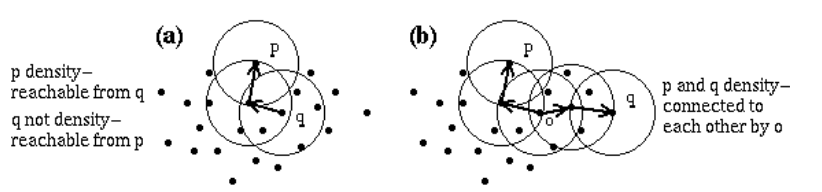
\includegraphics[width = 0.5\textwidth]{figures/dbscan_ester_1996.png}
  \caption{Example of DBSCAN selection showing how points are linked together. Figure curtsey of \cite{Ester96adensity-based}.}
  \label{fig:DBScan_example}
\end{figure}

The benefits of using parrallax compared to photometric data can be seen in \cref{fig:gaiaexample}. Where a usualy DBSCAN or HDBSCAN would remove stars that are off the main sequence the parrallax retains the non-mainsequence population. As this performs on a hierarchical basis the probablity of a star being part of a cluster is related to the 'distance' between the first ('birth') cluster and the last cluster ('death'). The persistance of a cluster is expressed as $\lambda = \frac{1}{\text{distance}}$, where distance is the distance from the core cluster. The persistance of birth and death is then $\lambda_{\text{birth}}$ and $\lambda_{\text{death}}$ respectively. \\ The stablity of a classified cluster is then 

\begin{equation}
  \text{stablity} = \sum_{p \in \text{cluster}} (\lambda_p  - \lambda_{\text{birth}})
\end{equation}

The probablity of a point in a cluster is then classified as the normalised corresponding stablity. The results of this classification can be found in \cref{tb: population_classification}. The uncertainty on the population is taken proportion of the population that had 80\% or less membership probablity. With the expected population taken from \cite{2020A&A...640A...1C} and in the case of Bochum 2 taken from \cite{1993Turbide}. 

\begin{table}[h!]
  \caption{Results of Gaia population classification.}
  \label{tb: population_classification}
  \begin{tabular}{lcc} \hline \hline 
    Target & Population & Study Population \\ \hline 
    Berkeley 28 & $79 \pm 17$ & 53\\ 
    Bochum 2 & $110 \pm 13 $ & 110 \\ 
    NCG 2324 & $251 \pm 26 $ & 242 \\
    NGC 2355 & $139 \pm 128$ & 261 \\ \hline 
  \end{tabular}
\end{table}


\begin{figure}
  \centering
  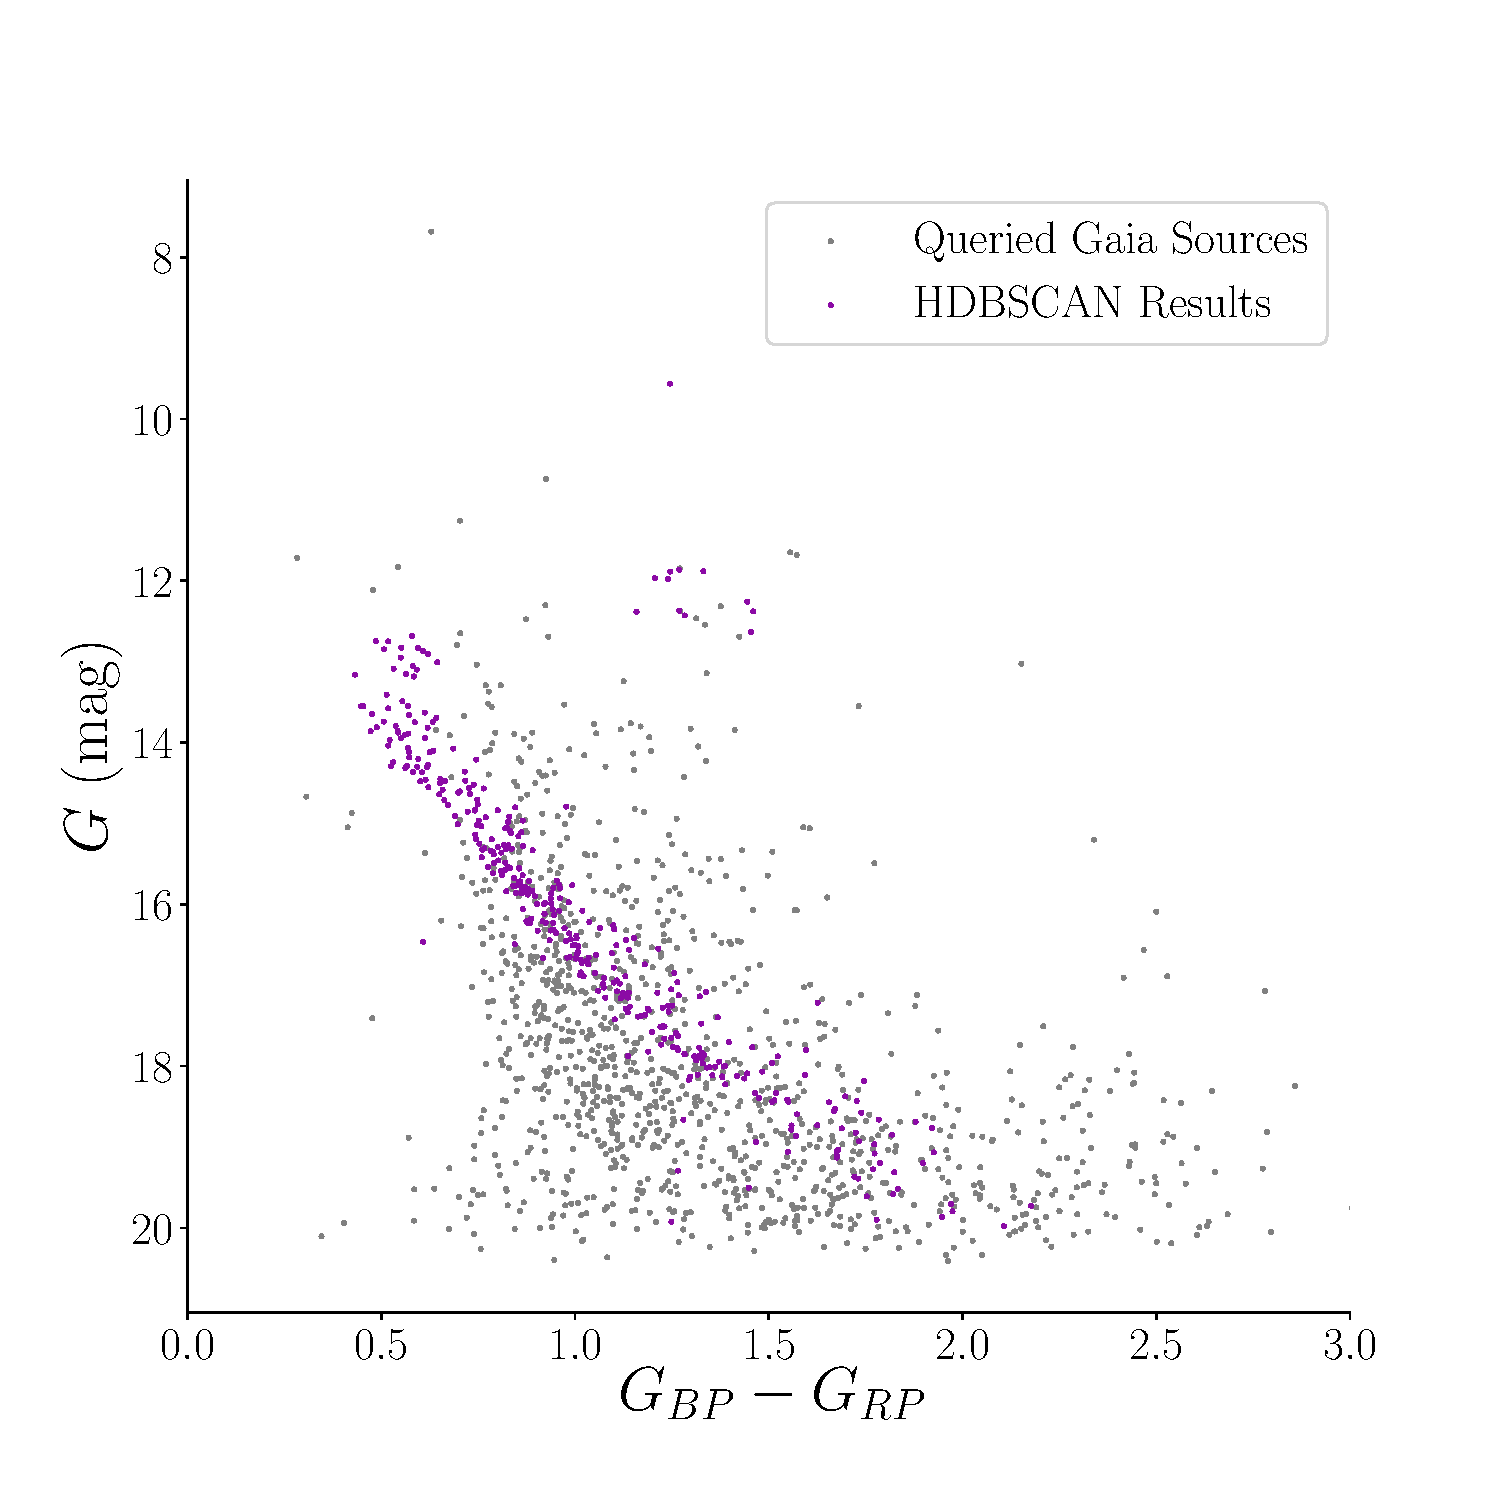
\includegraphics[width = 0.45\textwidth]{gaia_plot_example.pdf}
  \caption{Stellar population determined for NGC 2355 using Gaia parallax data and HDBSCAN method.}
  \label{fig:gaiaexample}
\end{figure}

Determining the population through the use of HDBSCANs and Gaia provided promisng results. Each cluster responded to the filtering with the underestimations seen in NGC 2123 impart due from stars with a magnitude of 19 or greater. However the calculated probablities had varying results in quantifying and uncertainty. For the more sparsely populated cluster such as Berkeley 28, Bochum 2 and NGC 2324 the probablities returned a mean memebership rate of 89\%, 92\%, and 95\% respectively. While these estimations appear adequate and are in line with the ranges shown for these clusters in similar studies \citep{2019A&A...623A.108B, 1988Mohan, 1998Frandsen, 1991Kalunzy} the population of each cluster should be around a $30\%$ underestimation given the distribtuion of brightness in each cluster. 

\section{Determining Cluster Parameters}

Following the cluster population analysis the next step is fitting parameters to the set of observed and proposed open-clusters. 

\subsection{Isochrones}
\subsubsection{Detailing MIST}
The isochrones generated for use in this study were created using the MESA Isochrones and Stellar tracks \citep[MIST;][]{2016ApJ...823..102C} from the Modules for Experiments in Stellar Astrophysics \citep[MESA;][]{2018ApJS..234...34P}. MIST uses the Sun as a basis for its chemical compositions, with solar abundances modelled by \cite{doi:10.1146/annurev.astro.46.060407.145222} with $Z_\odot = 0.014$. MIST  takes hot wind-driven mass-loss from \cite{2001A&A...369..574V}, cooled dust driven mass loss from \cite{1988A&AS...72..259D} and \cite{2000A&A...360..227N} for any mass loss in the helium star phase. With convection boundaries modelled after \cite{1947ApJ...105..305L} and convection overshooting modelled using \cite{2000A&A...360..952H}. \\

\subsubsection{Using MIST}
The choice of using MIST was due to its recent creation compared to WEBDA used isochrones (Padova \& Geneva) and also it's ease of interpolation oppose to other commonly used ioschrones like PARSEC. A detailed comparative studies of popular modern isochrones is carried out by \cite{2022MNRAS.512.5717A}. \\ 
Interpolation and plotting was carried out using a forked version of the \verb|isochrones| package created by \cite{2015ascl.soft03010M}. \verb|isochrones| posessed a high functioning front end for accessing MIST isochrones from the Johnson UBVI system and plotting with with minimal turnaround time. This allowed for quick incremental change in the parameters generating isochrones making the process for incrementally fitting isochrones less cumbersome. 


\subsection{Isochrone Results}

Isochrone fitting was carried out on 10 clusters as listed in \cref{tab:target_list}. The 4 observed clusters, Berkeley 28, Bochum 2, NGC 2324 and NGC 2355 along with the 6 proposed clusters. The resultant parameters from these fits can be seen in \cref{tab:isochrone_parameters}. \\ Each cluster's parameters were compared to both their corresponding WEBDA study and \cite{2020A&A...640A...1C} to comapre attain value. Of the 4 observered clusters the 2 youngest clusters Bochum 2 (Bo 2) and Berkeley 28 (Be 28) did not show any discernable main sequence. This can be clearly seen in \cref{fig:obs_CMDs}


% \subsubsection{Bochum 2}

\begin{figure}
  \centering
  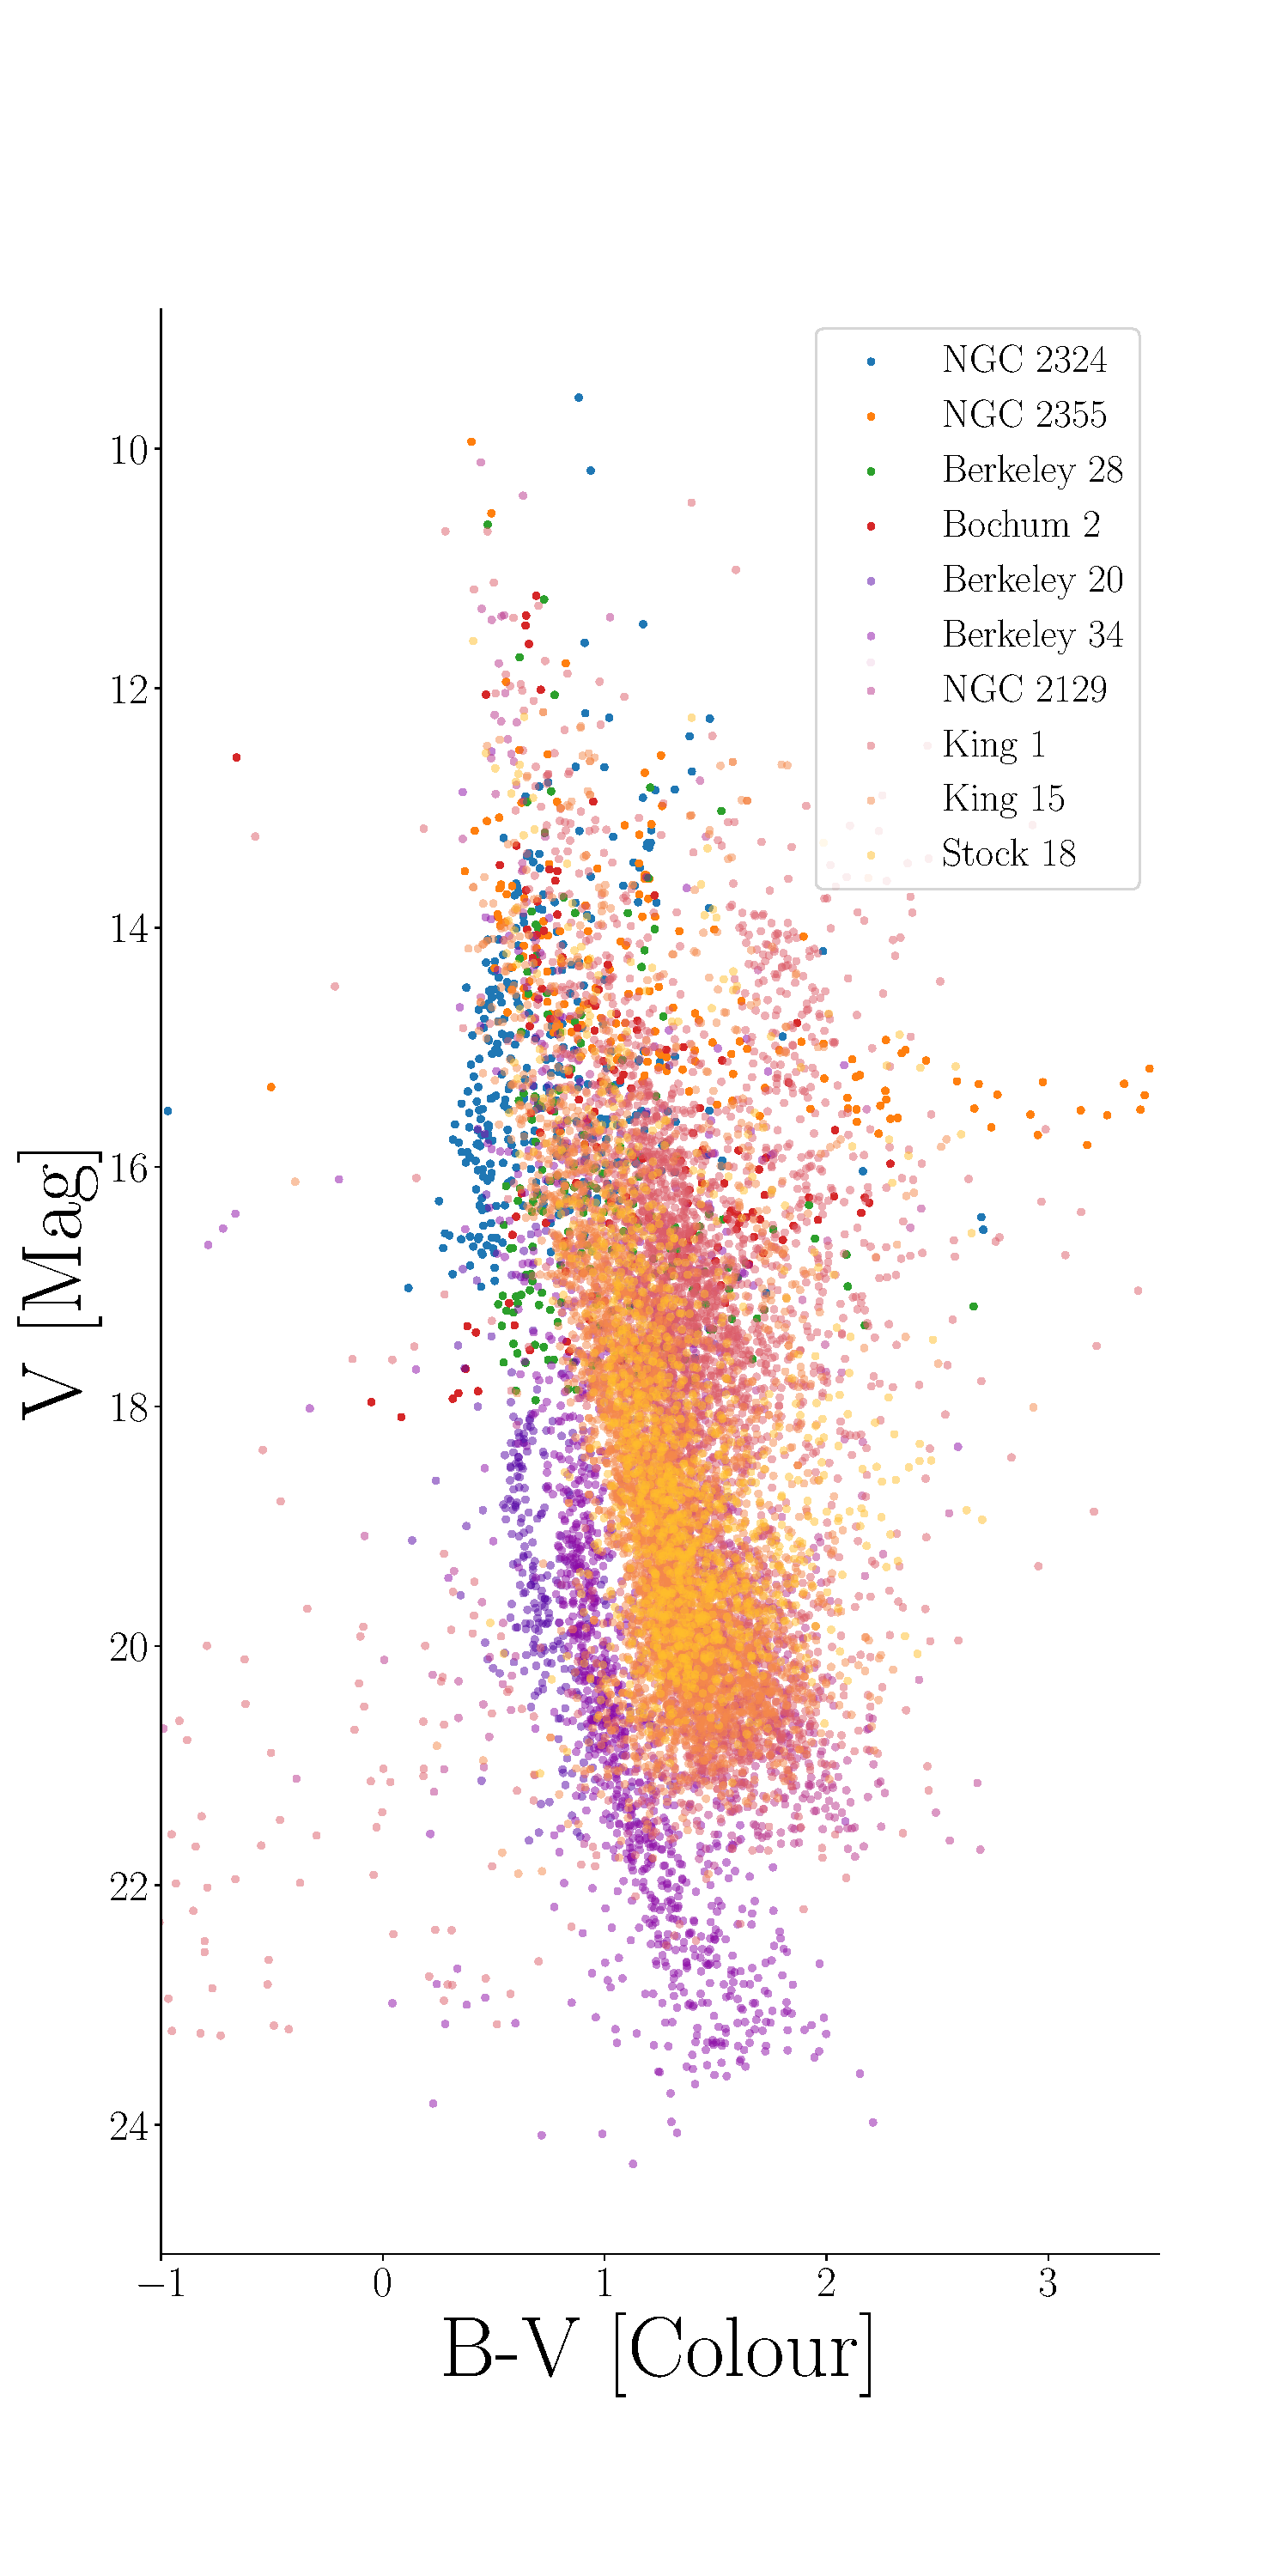
\includegraphics[width = 0.46\textwidth]{figures/master_cmd.pdf}
  \caption{Overall CMD plot of all stars analysed in this study. This illustrates homogenity of the stellar population distributed along the main-sequence. Each colour representing an open cluster.} 
\end{figure}

\subsection{Goodness of Fit}

Fitting isochrones in itself can be an unwieldy task and often difficult to quanitfy the 'goodness' of fit. In this case the isochrone was first fitted by varying values of colour to find the extinction in the V band using the following expression as per \cite[pg. 237]{dyson1980physics}. 

\begin{equation}
  A_v = 3.1 \; E(B - V)
\end{equation}

Distance was then determined taking into account the value for extinction. Both age and metallicity were determined by fitting various incremental parameters by eye and taken the 'best' fit as the parameters value. The errors were taken to be the limits where the parameters had argument for being a 'good' fit. While not a quantitative or rigorous method for justifying a data fit it has historically provided results with an adequate degree of confidence. The release of GDR2 has propmted a new wave of studies developing means of attaining a tangeible goodness of fit for modern ioschrones. \cite{2021A&A...649A.127V} has coined a promosing method of Mahalanobis distances of stellar data points to plotted isochrones and mask resultant synethic CMDs with $\chi^2$ distribtuions to fit to Gaia samples as a mean of seeing if a fit is good.



\begin{figure*}
  \gridline{\fig{isochrones/Berkeley28.pdf}{0.46\textwidth}{(a)}
            \fig{isochrones/Bochum2.pdf}{0.46\textwidth}{(b)}
            }
  \gridline{\fig{isochrones/NGC2324.pdf}{0.46\textwidth}{(c)}
            \fig{isochrones/NGC2355.pdf}{0.46\textwidth}{(d)}
            }
  \caption{Colour magnitude diagrams fitted to MIST isochrones of observational data with complementary WEBDA data plotted in grey. Histogram on each the x and y axis represent distribution of colour and magnitude respectively. }
  \label{fig:obs_CMDs}
\end{figure*}

\begin{figure*}
  \gridline{\fig{isochrones/Berkeley20.pdf}{0.46\textwidth}{(a)}
            \fig{isochrones/Berkeley34.pdf}{0.46\textwidth}{(b)}
            }
  \gridline{\fig{isochrones/King1.pdf}{0.46\textwidth}{(c)}
            \fig{isochrones/King15.pdf}{0.46\textwidth}{(d)}
            }
  % \caption{Colour magnitude diagrams fitted to MIST isochrones of observational data with complementary WEBDA data plotted in grey. Histogram on each the x and y axis represent distribution of colour and magnitude respectively. }
  % \label{fig:obs_CMDs}
\end{figure*}

\begin{figure*}
  \gridline{\fig{isochrones/NGC2129.pdf}{0.46\textwidth}{(e)}
            \fig{isochrones/stock18.pdf}{0.46\textwidth}{(f)}
            }
  \caption{Colour magnitude diagrams fitted to MIST isochrones of observational data with complementary WEBDA data plotted in grey. Histogram on each the x and y axis represent distribution of colour and magnitude respectively. }
  \label{fig:obs_CMDs_2}
\end{figure*}

% \subsection{Observation Results}

\begin{deluxetable*}{lcccccccccc}
  \tablecaption{Cluster parameters. \label{tab:isochrone_parameters}}
  \tablewidth{0pt}
  \tablehead{
  \colhead{Cluster} & \multicolumn{2}{c}{Age} & \multicolumn{2}{c}{Distance} & \multicolumn{2}{c}{Colour} & \multicolumn{2}{c}{Metalicity} & \multicolumn{2}{c}{Extinction} \\   
  \colhead{} &\multicolumn{2}{c}{Myr} &\multicolumn{2}{c}{$M_{V_0}$} & \multicolumn{2}{c}{$E(B-V)$} & \multicolumn{2}{c}{Fe/H} & \multicolumn{2}{c}{$A_v$} \\ \cline{2-11}
  & \textit{Obs.} & \textit{Study} & \textit{Obs.} & \textit{Study} & \textit{Obs.} & \textit{Study} & \textit{Obs.} & \textit{Study} & \textit{Obs.} & \textit{Study}
  }

  \startdata
  Berkeley 28 & $63^{+6}_{-13}$ &  & $11.9 \pm 0.5$ & & $0.1_{-0.05}^{+0.05}$ & & $0.2^{+0.1}_{-0.05}$ & & $0.31 \pm 0.16$ & a \\
  Bochum 2 & $5 \pm 0.2$ & & $13.2 \pm 0.4$ & & $0.64 \pm 0.1 $ & & $-0.02^{+0.005}_{-0.005}$ & & $1.98 \pm 0.31$ & a \\ 
  NGC 2324 & $427 \pm 0.5$ & & $13.2 \pm 0.05$ & & $0.26 \pm 0.03$ & & $-0.52 \pm 0.07$ & &  $0.81 \pm 0.09$ &  \\
  NGC 2355 & $676^{+3.44}_{-1.64}$ & & $11.6^{+0.06}_{-0.05}$ & & $0.31^{+0.06}_{-0.03}$ & & $-0.07 \pm 0.02 $ & & $0.96 \pm 0.12$ &   \\ \hline 
  Berkeley 20 & $6026^{+12}_{-12}$ & 5000 & $14.4^{+0.2}_{-0.3}$ & $15.1 \pm 0.8$ & $0.09 \pm 0.03$ & $0.13$ & $-0.35 \pm 0.05$ & -0.75 & $0.28 \pm 0.09$ & 0.403 \\
  Berkeley 34 & $2239^{+24}_{-24}$ & & $14.7^{+0.3}_{-0.1}$ & & $0.5^{+0.1}_{-0.1}$ & & $0.02 \pm 0.005$ & & $1.55 \pm 1.33 $ & a \\ 
  King 1 & $2455^{+52}_{-52}$ & & $11.2^{+0.5}_{-0.5}$ & &  & & & & & a \\
  King 15 & & & & & & & & & & a \\
  NGC 2129 & & & & & & & & & & a \\
  Stock 18  & & & & & & & & & & a \\
  \enddata
  \tablecomments{The above table contains the determined value for both observed and proposed clusters along with the relevant WEBDA collected data by authors outline in \cref{tab:target_list}. }
\end{deluxetable*}

% \clearpage


\section{Classification}

\subsection{Open Cluster Classification Scheme}

As open clusters span many different distribtuions in both density, size and stellar constituents. Open clusters can contain large stellar agglomerations to just a handfull of stars. While classification systems can vary based on the context of the study the scheme coined by \cite{1930LicOB..14..154T} sees promeinant use. \\ This scheme classifies cluster based on three factors of the stellar population. a) their range of brightness, b) degree of concerntration and c) star population in the cluster. The details of this classification scheme can be seen in \cref{tab:trumpler_scheme}. In this study each observed target is classified based on this scheme.

\begin{deluxetable*}{lll}
    \tablecaption{Trumpler classification scheme. \label{tab:trumpler_scheme}}
    \tablehead{
    \colhead{Range of Brightness} & \colhead{Degree of Concerntration} & \colhead{Cluster Population} \\
    \colhead{(a)} & \colhead{(b)} & \colhead{(c)} 
    % \colhead{Number} & \colhead{Number} & \nocolhead{Name} & \colhead{Type} &
    % \multicolumn2c{(kpc)} & \colhead{Constellation} & \colhead{(mag)}
    }
    % \decimalcolnumbers
    \tablewidth{0pt}
    \startdata
    1 - Majority of stellar objects & I - Strong central concentration (Detached) & p - Poor $(n < 50)$  \\
    show similar brightness. & (Detached) & \\ 
    2 - Moderate brightness ranges & II - Little central concentration & m - Medium $(50 < n < 100)$ \\
    between stellar objects. & (Detached) & \\
    3 - Both bright and feint stellar objects  & III - No disenable concentration & r - Rich $(n > 100)$\\ 
      & IV - Clusters not well detached  & \\
      & (Strong field concentration) & 
    \enddata
    \tablecomments{Where $n$ denotes the amounts the stellar population in a given cluster. For example Pleiades is a I3rn cluster and Hyades is a II3m cluster. Where the 'n' flag on a classification relates if the cluster shows nebulosity.}
\end{deluxetable*}

\subsection{Classification Results}

Each cluster was classified based on the distribution of V magnitude which can be seen on the $y$-axis of both \cref{fig:obs_CMDs} and \cref{fig:obs_CMDs_2}. With the concerntration of each cluster based on distribtuion of confirmed stars from the cluster's center. \\ 
The results of each classification can be seen in \cref{tab:trumpler_results}. Each cluster was deemed to match \cite{1981ADCBu...1...90L} and CITE JANES

\section{Supplementary Data for Tracing} \label{sec:supplementary_data}

This study directly uses 260 clusters cataloged by \cite{2020A&A...640A...1C} to aid the observational sample size. This study also uses a 269 cluster catalog by \cite{2019A&A...623A.108B} to use as comparison to determined observational parameters. When searching for studies to compliment this work use Gaia's second data release (DR2) was given preference. The reason for the use of supplementary data was to provide a more varying survey of the galactic disk. The first data set implented was 269 clusters analysed and catalogued by \cite{2019A&A...623A.108B}. This dataset contains large sample of clusters analysed from Gaia DR2, with each of the clusters containg a high degree homogenity amoung the stelllar population. The cluster populations were determined using Bayesian methods of statistics along with DR2 astrometric data. In doing this the probablity of each star being a member of each clusters was $70\%$ or greater. The parameters of each cluster was found using PARSEC isochrones \citep{2012MNRAS.427..127B}. This data set worked well to fill out a sample size in the galactic disk as seen in \cref{fig:TargetSelection}. Although this survey contained a good amount of clusters with varying age it lacked a lot of ancient clusters of the milkey way. To supplement this gap 260 old clusters from \cite{2020A&A...640A...1C} were used. This study used a neural network trained on high accuracy data sets to estimate cluster parameters using GDR2 parallax values and photometry $(G \leq 18)$. 

\subsection{Cataloging}

Stars that were confirmed as part of the population have been cataloged with their respective parameters and can be found in X. 


% Here the temperture of each star was determined using Ballesteros' formula with propagation of uncertainty carried from the error on both the $B$ and $V$ magnitude. 

% \begin{eqnarray}
%   \nonumber T = 4600 \; \text{K}  \; \left( \frac{1}{0.92 \; B-V + 1.7}  \right. \\
%   \left. + \frac{1}{0.92 \; B - V + 0.62}  \right)
% \end{eqnarray}


\begin{figure}[h!]
  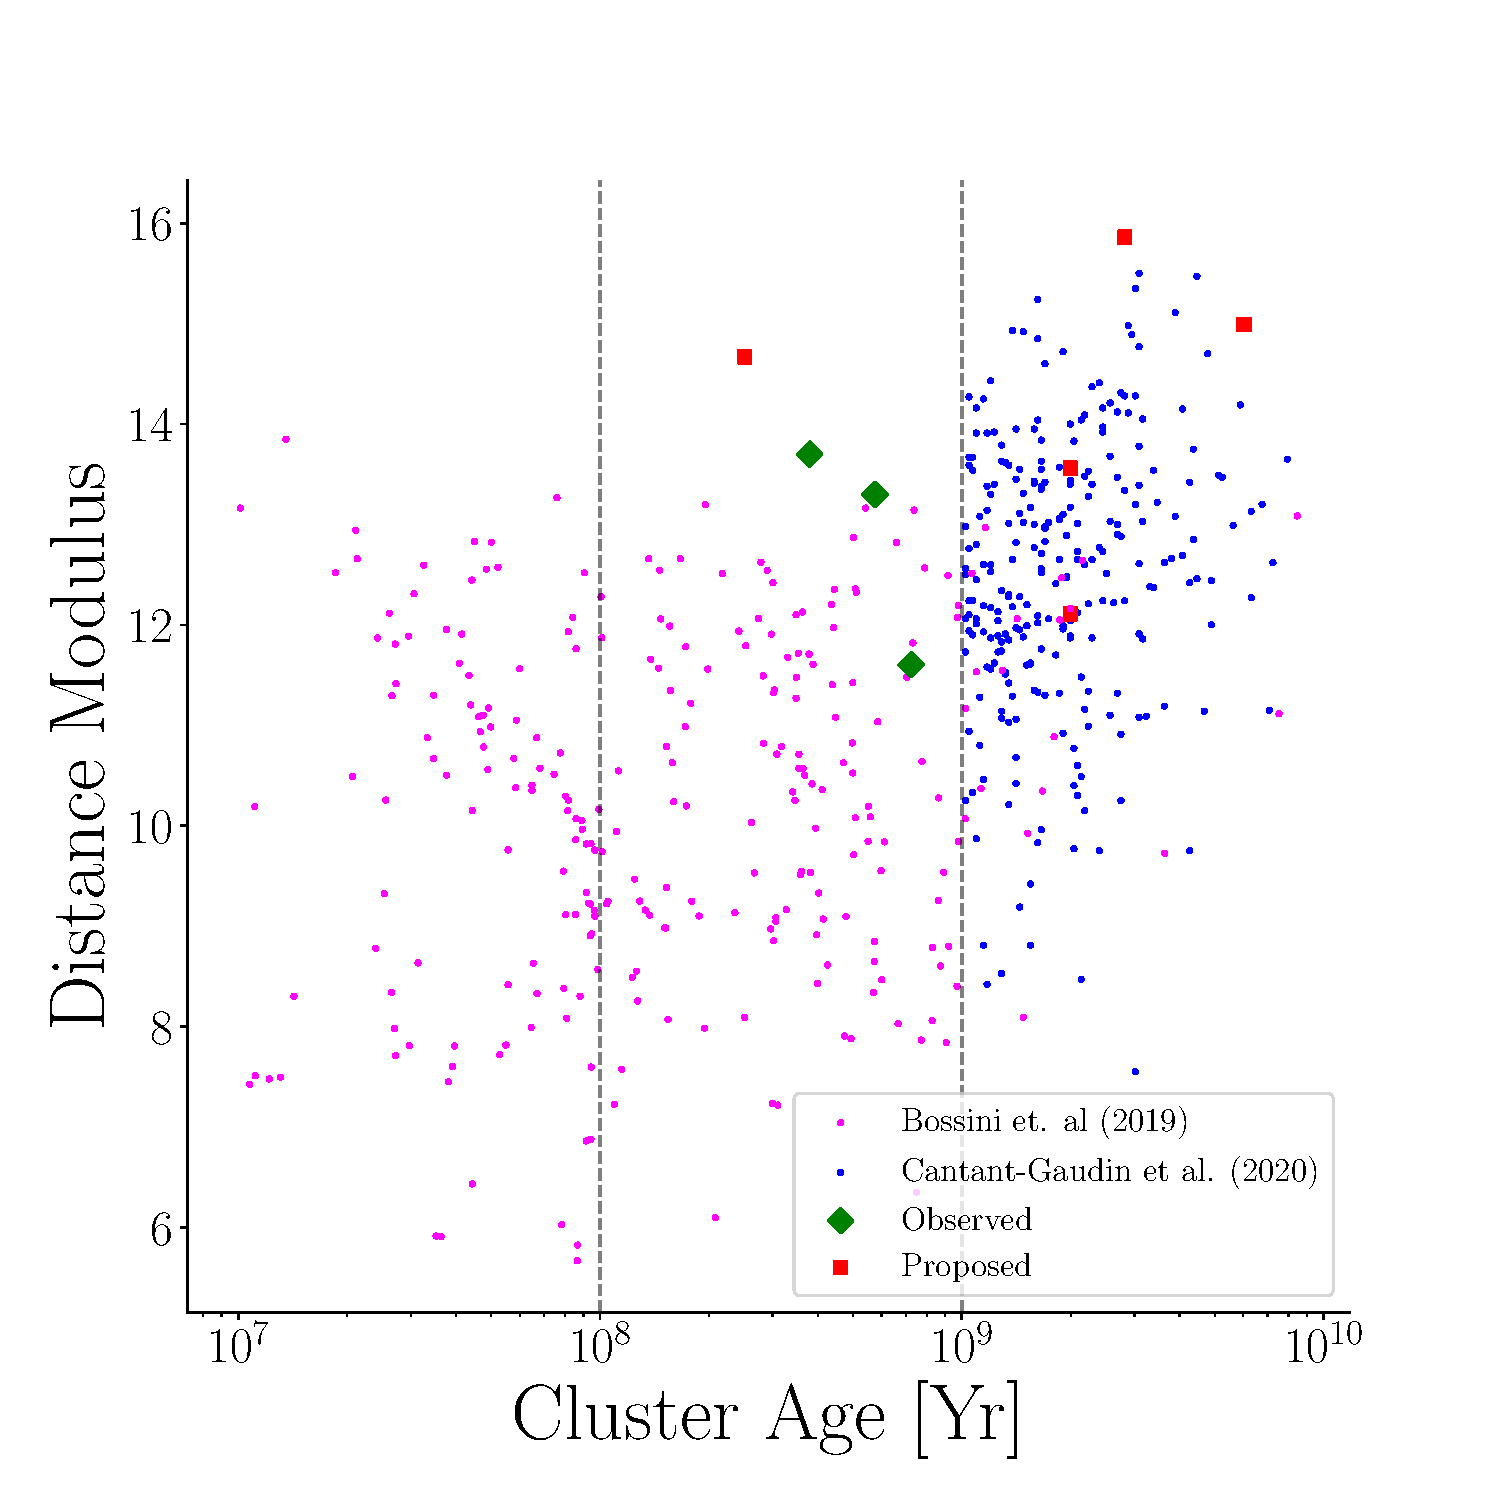
\includegraphics[width = 0.46\textwidth]{supplementary_data_plot.pdf}
  \caption{Distance against the log age of both observed targets, proposed targets and supplementary targets. This plot illustrates the gap of old clusters from \cite{2020A&A...640A...1C}'s data fills.   \label{fig:supplementarydatafig}}
\end{figure}


\begin{deluxetable*}{lccccc}[ht!]
  \tablecaption{Results of Trumpler classification on observed targets. \label{tab:trumpler_results}}
  \tablehead{
  \colhead{Target} & \colhead{$\Delta V_{mag}$} & \colhead{$\Delta B_{mag}$} & \colhead{$\sigma_c$} & \colhead{Population $n$} 
  }
  % \decimalcolnumbers
  % \tablewidth{}
  \startdata
  Berkeley 28  &  &  &  & $79 \pm 17$ & m \\ 
  Bochum 2 &  &  &  &   $110 \pm 13$ & r \\ 
  NGC2324 & 12 & 12 & 12 & $251 \pm 26$ & r \\
  NGC2355 &  &  &  & $139 \pm 128 $ & r \\ 
  \enddata
  \tablecomments{Where $n$ denotes the amounts the stellar population in a given cluster. For example Pleiades is a I3rn cluster and Hyades is a II3m cluster. Where the 'n' flag on a classification relates if the cluster shows nebulosity.}
\end{deluxetable*}

\begin{figure*}[ht!]
  \gridline{\fig{figures/target_selection.pdf}{0.8\textwidth}{}
            }
  \caption{Aitoff projection of targets in terms of galactic co-ordinates, longitude ($l$) and laititude ($b$). Targets observed at CAHA are observed in X, the orginal proposal targets shown in X and studies by \cite{2019A&A...623A.108B} and 
  \label{fig:TargetSelection}}
\end{figure*}
  
\section{Galactic Tracing}

Following the classification of the four observed clusters and parameterising of the 10 clusters both proposed. They're age and location was used to make an enquiry into the present shape of the galactic disk. Here \cite{2020A&A...640A...1C} sample of old open clusters is used fully. A preliminary caveat is the use of the term 'inner-disk'. For this work as with similar studies the inner-disk is taken to be clusters that fall within a galacto-centric distnace smaller than the Sun. This value\footnote{Currently the most accurate accepted value for solar distance to Sagittarius A*} is taken to be $8180 \pm 35$ pc given by \cite{2018A&A...616A...1G}.

\subsection{Distribution of Old Clusters}

The sample size collected for this study includes old open clusters from across the galactic disk at varying distances as seen in \cref{fig:TargetSelection} and \cref{fig:supplementarydatafig}. Plotting the distribtuion of these clusters can be seen in \cref{fig:oc_dist}. \\ The immediate takeway from this depection is the lack of older open clusters within the innerdisk. Out of the 265 old clusters present only 62 (23.8\%) reside within the inner galactic disk. Moreover looking at the distribtuion of ages for as a function of both galocentric radius 

\begin{figure*}[ht!]
  \centering
  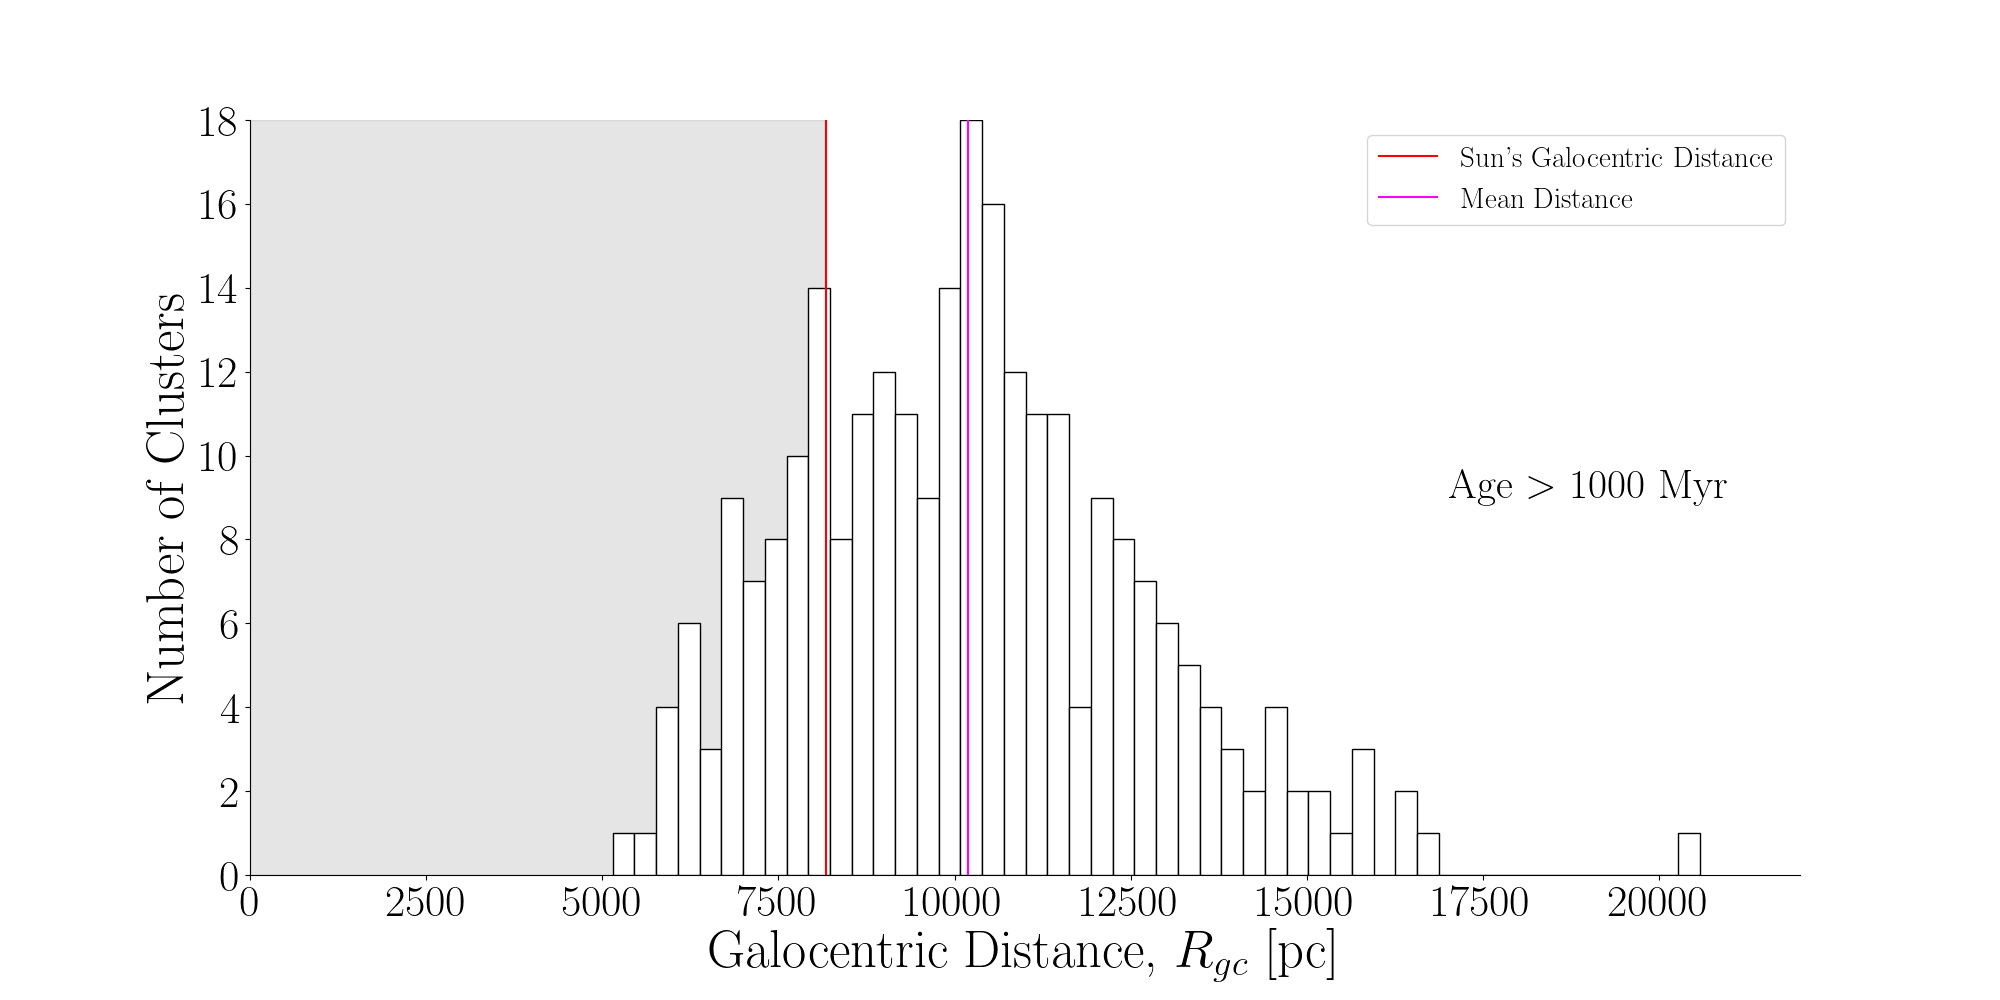
\includegraphics[width = \textwidth]{figures/opencluster_distribution.png}
  \caption{Distribution of old clusters according to galocentric distance. This sample includes 10 clusters of this work and 260 old open clusters from \cite{2020A&A...640A...1C}. The inner disk region is shaded. } \label{fig:oc_dist}
\end{figure*}

\subsection{** Reasons for Underabundance} \label{sec:rea4abunda}

Trying to determine a reason for the underabundance seen in older open cluster in the galactic inner disk has been a question since the start of using open-clusters in galactic tracing. \cite{1950BAN....11...91O} assumed uniform star formation in the disk and intially deemed it to be a case of extrapolation of younger clusters as open cluster which were much less prominent by nature. \\ The most intutive explanation would that over time both gravatiational pull and destructive tidal forces would cause any open cluster to be pulled apart and dissapate into other surrounding objects through a long term interactions. \\ \cite{1973SvA....16..837K} derives a model for the evapouration of stars from open clusters based on mass distribtuion of opencluster and applies the model to the Pleiades predicting that all opencluster eventually dissapate. More recently \cite{2019A&A...624A...8A} confirmed the decline in stellar population in 6 open clusters. This distribtuion is based on dynamic simulations of age, limiting radius, stellar mass, and velocity dispersion. Looking outside the realms of internal dynamics in the cluster causing dispersion there is also interactions with other objects in the galactic disk causing an acceleration of cluster degeneracy. The primary suspect in these disruptive interactions is massive dust cloud in the galactic core as first noted by \cite{1958ApJ...127...17S}. Here it was stated that for a cluster of a mean density of $M_\odot/\text{pc}^3$ the dispersion time would be $\sim 200 \; \text{Myr}$. Such that lower mass clusters would dispers at a much faster rate. \\ 
While the precessing arguments have both logic and evidental basis for these findings and open cluster do increasingly disperse with time. There are few contradictory points of interest. 

\subsection{Relating Cluster Age to Galactic Position}

The intresting consideration is that despite the internal and external interactions discussed in the previous section there is still a apperciable amount of older clusters close to the galactic disk. Berkeley 17 (10 Gyr) and Collinder 261 (8 Gyr) are both within 200 pc of the plane. As \cite{2020A&A...640A...1C} discusses since the release of GDR2 confrimation of 9 old clusters\footnote{NGC 6005, NGC 6583, UBC 307, UBC 310, UBC 339, LP 866, UFMG 2, Ruprecht 134, and Teutsch 84} within $R_{GC}< 6500 \; \text{pc}$. 
Small parallax coupled with sparse CMDs as illustrated by Be 28 indicate that there could be more clusters located deeper in the disk within this region, but difficulty inferring thier parameters prevents meaningiful estimates of distance.  \\ While the first large scale catalogs of open clusters by \cite{lynga1982open} and \cite{dias2002new} suggest that destructive forces are too effcient to relate to the amount of older clusters currently seen. 

\begin{figure}[ht!]
  \centering
  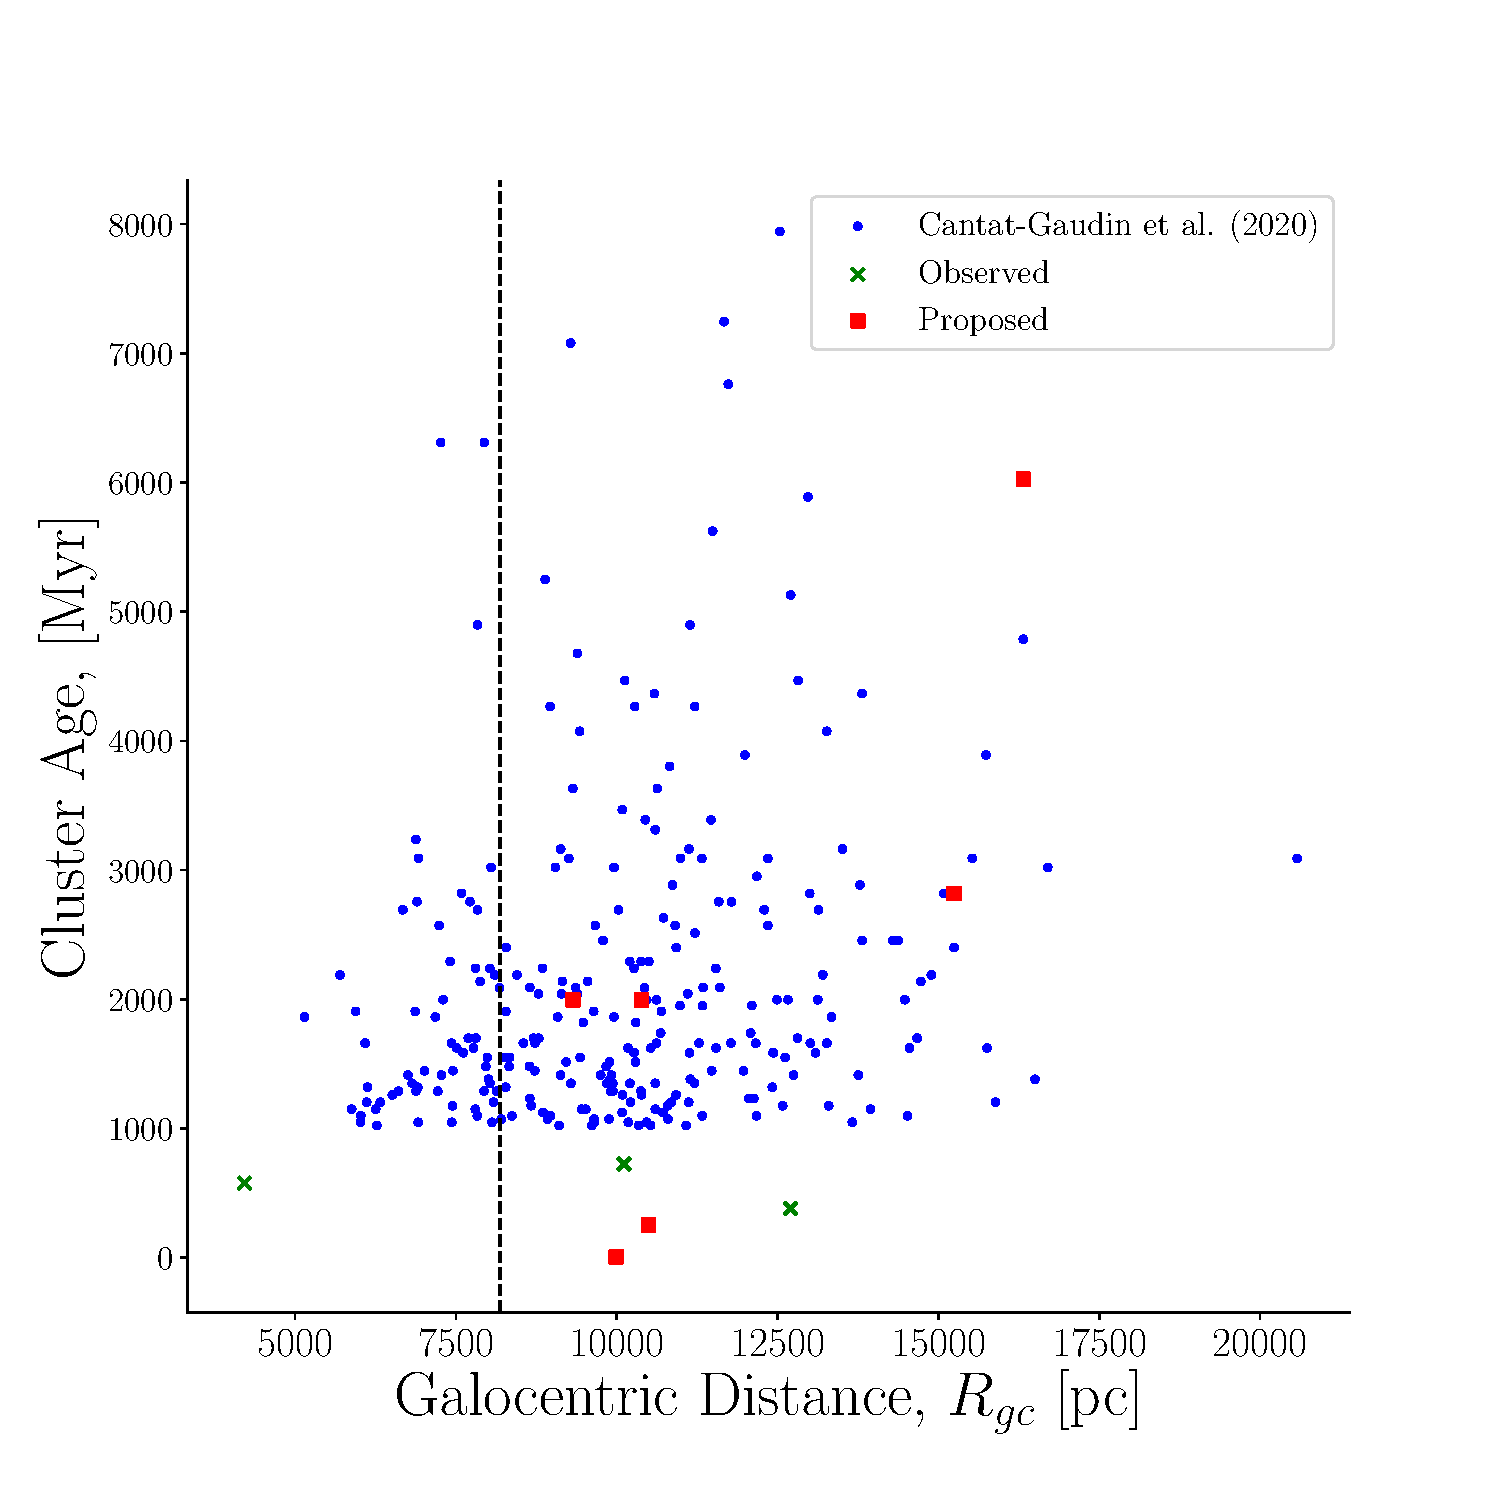
\includegraphics[width = 0.46\textwidth]{figures/agevsrgc.pdf}
  \caption{Plot of cluster age against distance galocentric distance, $R_{\text{gc}}$}
  \label{fig:agevsrgc}
\end{figure}

\Cref{fig:agevsrgc} shows no clear relationship between the age of a given cluster and its galocentric distance. As shown by \cref{fig:oc_dist} most of the old clusters lay outside the innerdisk with 4 of the clusters under 1000 Myr also situated outside the innerdisk. When looking at \cref{fig:agevszpos} there is also no clear relationship between age and cluster presence in the bulge. The extreme outliers of clusters like Be 20 could be residual formation from an interaction of more populas clusters near the bulge. \\ Given these factors it is likely that the relationship between cluster age and position in the galactic plane is a nuanced relationship between inherent cluster properties, internal dynamics and the overall enviroment in the galaxy. \\ An extension to this study would be to use GDR2 to investigate the orbits of old and ancient open clusters. It has been shown in studies X and X that older open clusters adhere to extensive ellpitcal orbits. If these orbits were simulated on a large enough time-scale it could show a migration pattern into the inner-disk. It would also be worth-while to further explore the internal dynamics of the cluster, finding a relation between intial-mass of older open clusters and the strength of their gravatiational bounds.

\begin{figure}[ht!]
  \centering
  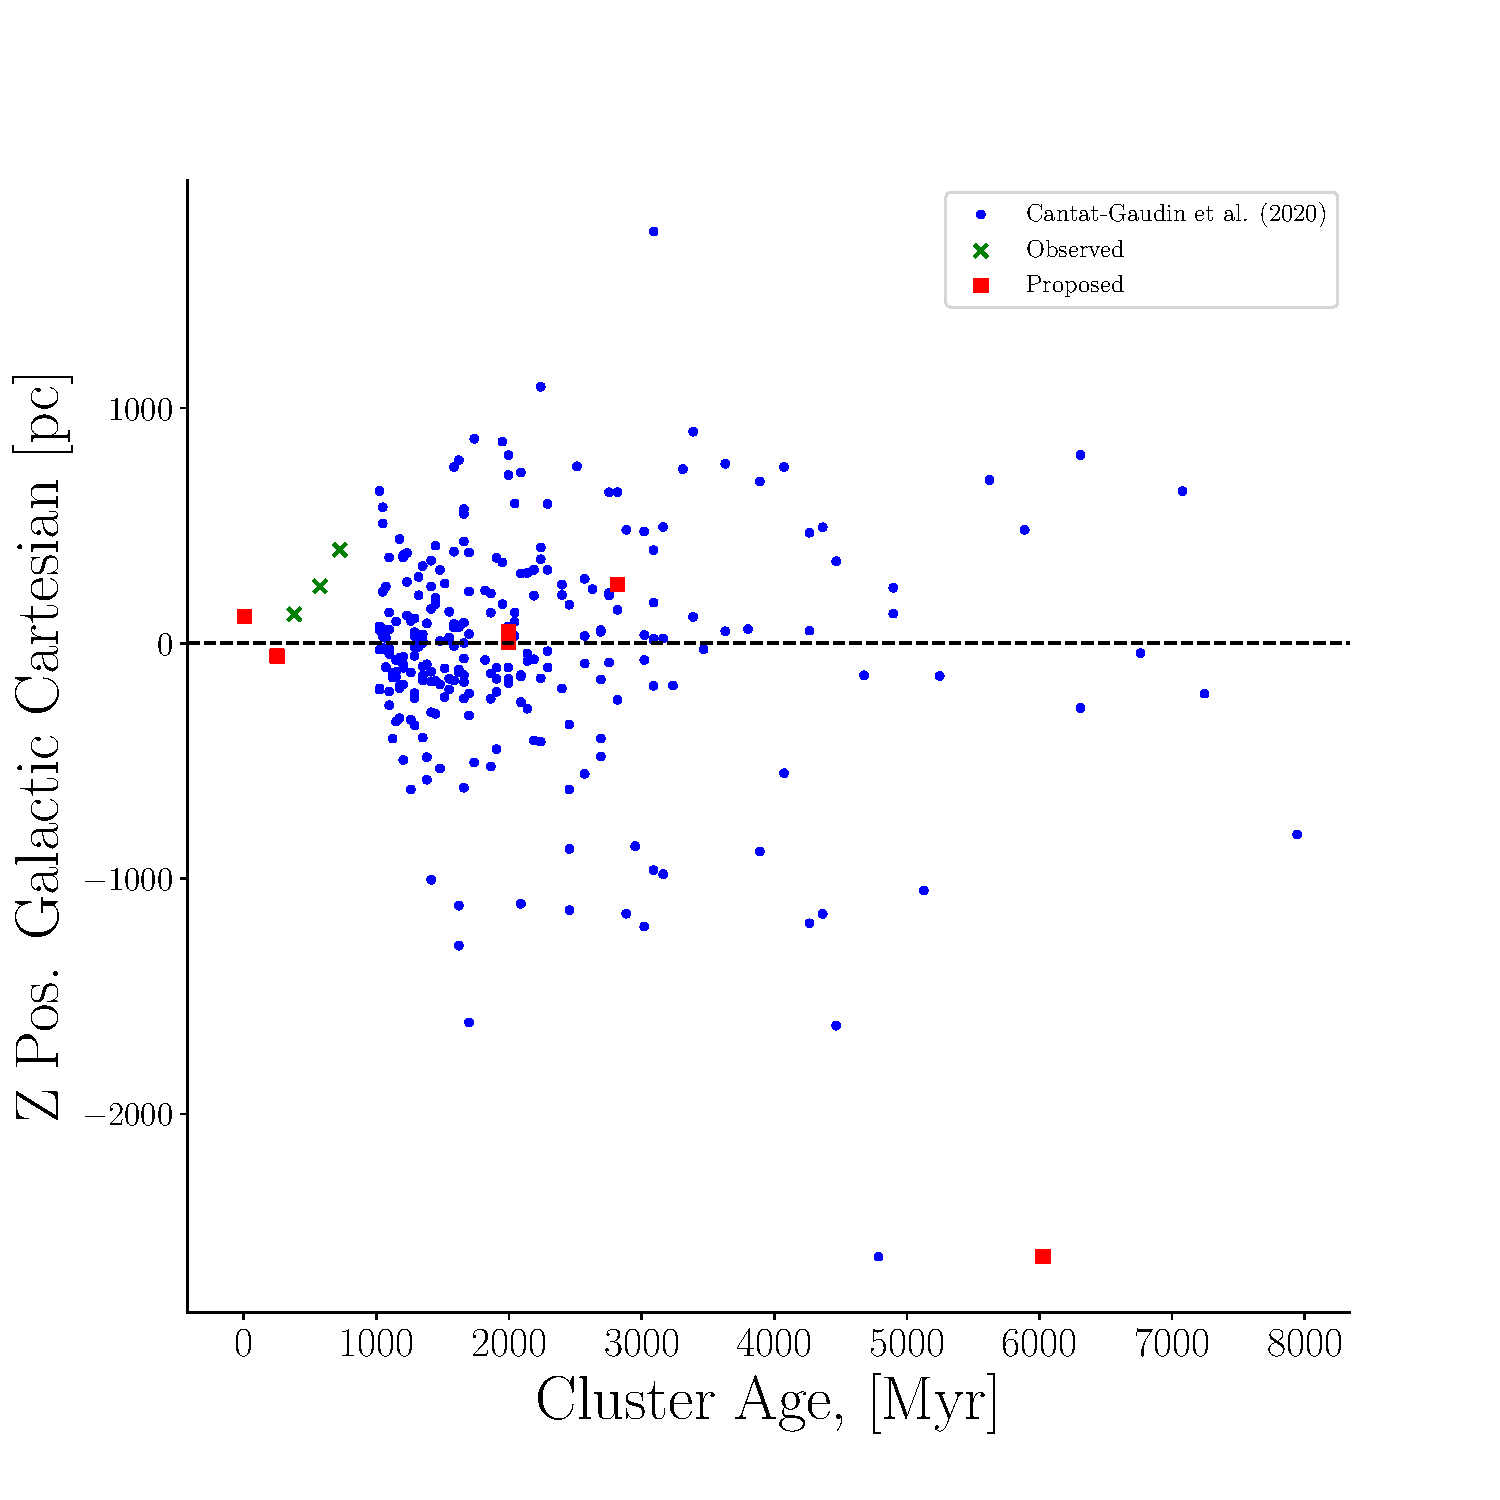
\includegraphics[width = 0.46\textwidth]{figures/agevszpos.pdf}
  \caption{Plot of cluster age against galactic cartesian co-ordinates in the z-direction, $Z$.} 
  \label{fig:agevszpos}
\end{figure}


\subsection{Galatic Evolution}

As there is a substatial amount of older clusters found throughout the disk with evidence of a substatial surival rates. The disk indicates a thincking of the galactic disk with increased galocentric distance. The excursion of old open clusters to larger galocentric distances away from disruptive appears to be highly assymetric. There also could be observational selction at play as previosuly stated with asterism and difficulty differentating older clusters from concerntrated areas in the disk. These findings are also echoed in \cite{2006Bon}. 

\section{Conclusions}

This study collect UV data on four clusters from the WEBDA catalog. Each observed cluster was classified based on exclusively Gaia's second data release through hierarchical density based scanning. Each cluseter was characterised using MIST isochrones and supplemented using DSEP isochrones. The observed clusters were then classified based on the Trumpler classification scheme and cataloged. \\ 
Additionally a further 6 clusters of intrest were also charactersed using MIST isochrones. Each cluster showed resultant parameters that fell within expected range of either their relevant WEBDA study or entry in the collected supplementary data. Any large invariance due to the the lack of definition on the main-sequence (Be 28 and Bo 2) and smaller variance expected due to the fitting of modern isochrones.

\section{Third Party Software and Catalogs} \label{sec:cite}

This work made use of a variety of software suites and python modules. \href{https://github.com/ejeschke/ginga}{Ginga} was used as the primary image viewer and used as reference when performing photmetry.  \\ All data and processing files can be found on the author's \href{https://github.com/OwenJohnsons/Open-Clusters-Project}{GitHub}.